\section{Results}
\subsection{Do the admission rules disagree?}
Figure~\ref{fig:frontier} establishes both directions in the deterministic map. The certificate's model-derived radius can be smaller than the fixed margin in one regime and more restrictive in another. It is not uniformly a looser or stricter version of the guard. The causal experiment further changes the distribution of starting measurements: a three-sample residual trigger selects measurements from the anomaly tail. Consequently deterministic band membership does not guarantee that every causal trajectory reaches the mapped admission state.

\subsection{Paired causal confirmation and controls}
Table~\ref{tab:matched} gives all six settings for all four methods, preserving the original two-selector counts and separating the later extension. At region~1's midpoint, the certificate selects 600/600 probes and accepts 594/600 fits, whereas the guard selects none. The paired acceptance-fraction difference is .990; the original descriptive 95\% interval is $[.970,1.000]$, with approximate six-setting adjusted limits $[.960,1.000]$. This is additional diagnostic access under the specified assumptions, not faster recovery of a failed link.

The controls show how selected states affect admission: the certificate selects 221 below the first band midpoint and 600 above it; the guard selects zero below and 239 above. At the reverse midpoint, the certificate refuses every probe while the guard selects and accepts 41/600. The reverse below control gives 28 guard acceptances; above, neither method triggers or selects. No guard-only admission in this study exhibits sampled outage, so it cannot be described as demonstrated unsafe. Every row has zero actual sampled outage and zero measured probe-induced sampled outage. This selected simulated population does not provide a physical reliability rate.

\begin{table*}[t]
\caption{All matched settings, each with 100 seeds and six fixed actual models ($n=600$ per row). S: selected probes; A: accepted completed fits; C: accepted offsets outside approximate radius; I: incomplete probes at 14~s. ES has no fit output (dashes). O is mean actual sampled outage after 2~s; E is mean angular excitation. The filter/ES rows are a later, separately frozen extension, not jointly predeclared confirmation.}
\centering\small\setlength{\tabcolsep}{10pt}
\begin{tabular}{llrrrrrr}\toprule
Setting & Method & S & A & C & I & O (s) & E ($\mu$rad$^2$ s)\\\midrule
\MatchedRows
\bottomrule\end{tabular}
\label{tab:matched}
\end{table*}

\subsection{Certificate scope and numerical replay}
Across the original confirmation, 1,421 UAD probes have calculated bounds and complete within-premise histories, with zero observed bound violations. There are no out-of-model or unverified UAD bound records in this particular dataset. The 7,200 new baseline records are noncertificate or no-probe records; they do not enlarge that count. Shadow replay exercises 204,624 monitor samples from those UAD probes without an observed breach. This is a check of supplied simulation evidence, not a closed-loop fallback demonstration.

The original separate replay covers 5,040,000 actuator steps with maximum absolute state-coordinate discrepancy $3.39\times10^{-21}$. The new extension independently replays another 5,040,000 steps with maximum discrepancy $1.36\times10^{-20}$. Across the two studies this is 10,080,000 checked steps. The unit audit also agrees exactly on 2,100 direct kernel sensor samples. These numerical agreements support consistency between source, saved trajectories and the independent calculation. They are neither a floating-point rounding proof nor evidence of a calibrated physical terminal.

\subsection{Estimator reliability and confidence misses}
At the first midpoint, 26 of 594 accepted UAD offsets lie outside the reported approximate radius (4.38\% of accepted fits). Six completed fits are rejected. The median accepted absolute gain error is $2.50\times10^{-4}$, but good gain estimates do not prove every offset or fault label correct. Conditional coverage after fitting and acceptance is not the exact-regressor calculation used to motivate the radius.

The difference has identifiable modeling reasons: regressors contain encoder noise; the log of multiplicative power noise is only approximately Gaussian; angle-noise variance and mean corrections are truncated approximations; feasible GLS uses estimated weights; and residual/radius selection changes the population of accepted records. This list explains why exact 95\% coverage cannot be transferred. It is not an attribution of each observed miss to one isolated cause; such causal attribution would require additional controlled ablations. The observed rate does not itself demonstrate calibration. In particular, the service theorem does not condition on the estimated covariance and cannot repair estimator bias.

The median trace-median UAD power slack at the same midpoint is $0.657657p_{\min}$. This substantial conservatism reflects separate worst cases in initial error, divergence, gain decline, finite-model motion and sensor event. The bound serves as a permission test rather than an accurate predictor of instantaneous received power.

\subsection{Premise violations and sensitivities}
A separate preserved 50-seed affine-drift sensitivity dataset is summarized consistently in Fig.~\ref{fig:sensitivity}; it is not pooled with the admission-frontier study. With nominal sensing UAD accepts 46/50 fits and one misses its approximate radius. Injecting unmodeled angle bias $[2,-1]\um$ gives 39 accepted fits; all 39 miss the radius and exceed $1\um$ actual error. Scaling the declared noise levels by five leads to no accepted UAD fits. The latter is abstention in this dataset, not proof that any unmodeled disturbance will be detected.

Bias also has a structural explanation. If $q_m=q+\beta$, then $q+b=q_m+(b-\beta)$; scalar optical power cannot distinguish the true offset from the shifted offset. Small residuals cannot resolve the ambiguity. Separate equal-variance Student-$t_5$ sensor-event stress gives 997 global event failures in 1,000 missions and 477 false acquisition indications under an adversarial minimum-time selector. That stress is not the optical plant trigger; it demonstrates that a Gaussian quantile cannot be transferred merely because variance matches.

Continuous actuator-grid tests are empirical stress only, not a continuous-parameter proof. Rapid gain variation and offset changes during a probe can violate A1--A2, and known bound failures in those distinct sensitivity records must remain out-of-model. Table~\ref{tab:violations} states what each failure mode permits one to conclude without treating successful interior samples as a theorem.

\begin{figure}[t]
\centering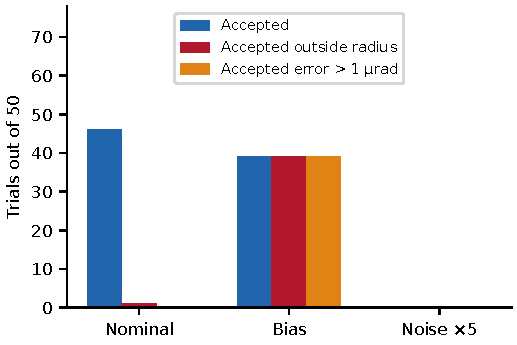
\includegraphics[width=\columnwidth]{premise_sensitivity.pdf}
\caption{Separate preserved affine-drift sensitivity, 50 paired seeds per condition. Counts are rebuilt from per-run rows into one table. ``Outside radius'' and ``error above $1\um$'' are different endpoints. This dataset is not the low-noise, nondeclining-gain confirmation.}
\label{fig:sensitivity}
\end{figure}

\begin{table}[t]
\caption{Premise failures and evidence-supported response. Refusal requires available evidence; an unmodeled violation can remain undetected.}
\centering\footnotesize
\begin{tabular}{@{}p{.27\columnwidth}p{.66\columnwidth}@{}}\toprule
Issue & Consequence / observed or analytic scope\\\midrule
Angle bias & Violates zero-bias contract; 39/39 accepted biased fits miss radius in separate sensitivity. Residual may remain small.\\
Heavy tails & Gaussian mission quantile invalid; adverse-time stress fails event calibration. No tail-robust theorem.\\
Between-set actuator & Interface refuses declared nonmember. Grid success does not certify a continuum.\\
Changing offset / faster gain loss & Breaks reference identity/window lower slope. Historical failures are retained as out-of-model.\\
Possible clamp activation & Linear RK4 enclosure unavailable; reject candidate. Simulations with clips do not extend the theorem.\\
Expired / incomplete evidence & Failure-closed metadata refusal; authority must establish truth of references.\\
Late mission start & New wrapper refuses insufficient remaining horizon. Baseline experiments retain 30 incomplete probes per method at reverse midpoint.\\\bottomrule
\end{tabular}
\label{tab:violations}
\end{table}

\subsection{Related architecture comparisons}
At region~1's midpoint, parameter KF selects and accepts all 600 fits, with 15 accepted offsets outside its approximate radius. Mean angular excitation is $74.747\ \mu$rad$^2$~s, versus 8.331 for UAD. The observed acceptance difference favors the filter; the excitation difference favors UAD in these settings. Neither covariance is exact, and the different waveforms and acceptance rules prevent attributing the difference solely to estimator architecture. Both have zero outage here, so no service-performance superiority over the filter is established.

At the reverse midpoint, parameter KF selects 558 probes and completes/accepts 528 fits. The remaining 30 are still probing at the mission end, not rejected fits. ES also selects 558 with 30 incomplete, and its completed trajectories are tracking results without diagnostic fit acceptance. At the first midpoint, ES angular excitation is 42.381, again with zero observed outage. Figure~\ref{fig:matched} compares common measurable endpoints without rewarding tracking as correct diagnosis.

Faithful comparisons with the original published constrained-AFD or safety-filtered-ES systems remain incomplete. The public guaranteed-AFD implementation \cite{massacode} is identified, but its CORA/solver dependencies are unavailable on the active path. The supplied dependency audit and mapping notes make this blocker explicit. The present KF and ES are conventional adapted architectures; they must not be represented as full reproductions of \cite{guo,massa,safees}.

\begin{figure*}[t]
\centering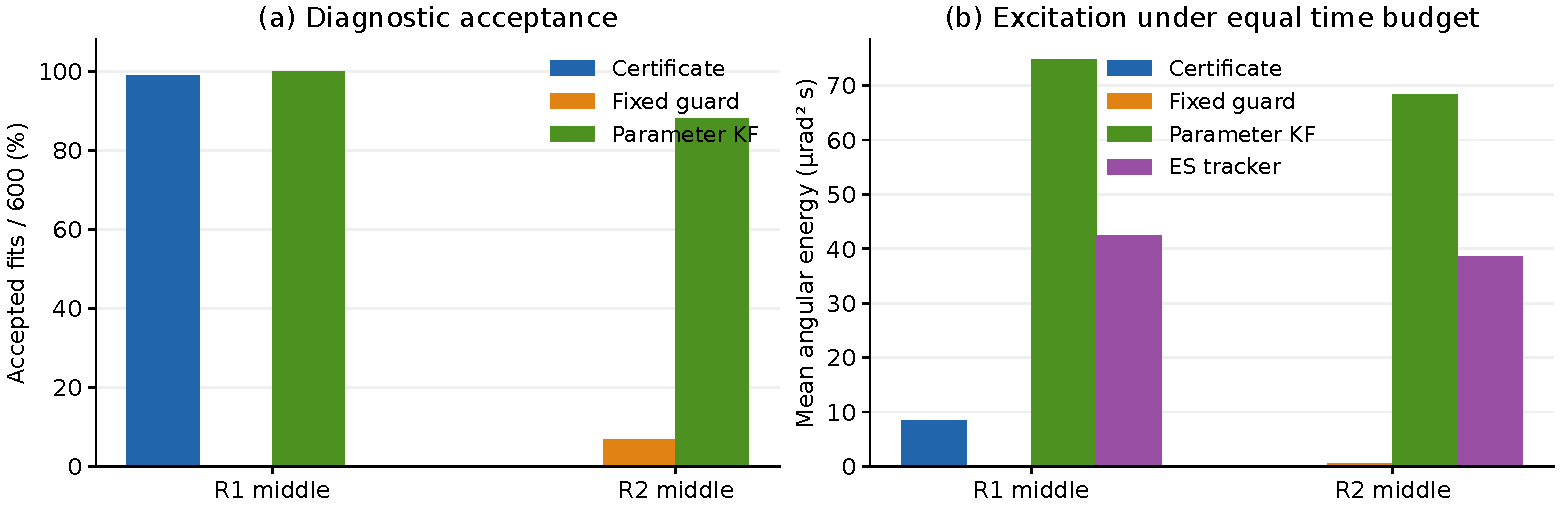
\includegraphics[width=\textwidth]{matched_confirmation.pdf}
\caption{Midpoint comparisons under the same maximum 2.88-s excitation time. Accepted-fit rates and angular excitation are different endpoints. ES is shown only for excitation because it does not produce diagnostic fits. All methods have zero sampled outage in these settings. Full below/above controls and completion counts appear in Table~\ref{tab:matched}.}
\label{fig:matched}
\end{figure*}
